\subsubsection{Clemmys --- Spotted Turtle}
\begin{center}
\begin{longtabu} to \textwidth {| | p{3.5cm} | X | |}

	\hline
	Taxonomy/Ancestry &
	\begin{itemize}[noitemsep]
		\item 1 N. American species, \emph{C. guttata}
		\item until recently, consisted of 4 species --- bog turtle, spotted turtle, western pond turtle, and wood turtle --- but recent genetic analysis revealed spotted turtle was distinct
		\item bog/wood turtles moved to \emph{Glyptemys}
		\item western pond turtle renamed \emph{Actinemys}
	\end{itemize}
	\begin{center} 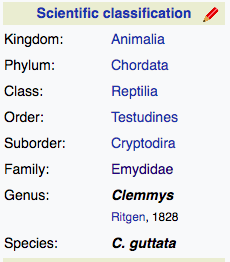
\includegraphics[scale=0.5]{testudines/emydidae/clemmys/tax} \end{center}
	 \\
	\hline
	Size & 
	8-12 cm (3.1-4.7 in)
	\\
	\hline
	Color &
	the carapace can be black, bluish-black. up to 100 small yellow round spots w/ the amount depending on range. the spotting pattern extends out to the neck and limbs from the head. the left side typically has more spots than the right. southern individuals tend to have smaller spots than northern. the plastron is yellow or orange-yellow w/ black spot present on each scute; w/ age, melanin of plastron increases until completely black.
	 \\
	\hline
	Anatomy &
	\begin{itemize}[noitemsep]
		\item lacks a keel
		\item small, semi-aquatic turtle
	\end{itemize}
	 \\
	\hline
	Dimorphism & 
	can be told apart from birth.
	
	males have a tan chin, brown eyes, and a long thick tail w/ a concave plastron.
	
	females have a yellow chin, orange eyes, a shorter tail, and a convex or flat plastron. they grow larger and have more spots.
	\\
	\hline
	Behavior & 
	\begin{itemize}[noitemsep]
		\item very intelligent; proven to have the intelligence of a mouse
		\item spends a lot of time on land; often basks on patches of grass near water
		\item only active in the cooler spring months; activity peaks during April-May
		\item in the warmest parts of summer (water temp. $> 30^\circ$C, they may aestivate terrestrially or aquatically for long periods of time, but they are relatively tolerant of drought conditions. burrow into leaf litter, marsh edges, open fields, or muskrat burrows
		\item winter dormant period may commence in later summer or fall
		\item distinct seasonal movement patterns
			\begin{itemize}[noitemsep]
				\item spring --- positive association in wetlands hosting abundant wood frog egg masses 
				\item late summer --- negative association in forested wetlands
			\end{itemize}
	\end{itemize}
	\\
	\hline
	Habitat & 
	variety of habitats including swamps, bogs, fens, marshes,  and wet pastures. can live in brackish environments including streams influenced by tides and vernal pools. avoids artificial reservoirs and deep open-water areas. habitats must have areas of soft substrate and at least some aquatic vegetation for survival.
	\\
	\hline
	Distribution & 
	ranges from southern Maine, Quebec, and Ontario, south along eastern US to Florida in east and central Ohio in west. disjunct populations in Canadian portion of range and in central Illinois, central Georgia, N./S. Carolina, and Indiana. despite large numbers of populations in Canada, many are not self-sustaining b/c they are small and isolated from each other. range overlaps that of many other turtles including wood, bog, snapping, painted, Blanding?s, eastern box, common musk, and eastern mud turtles.
	
	\begin{center} 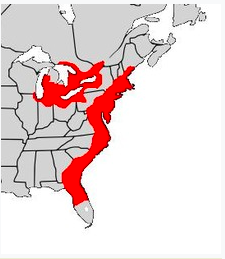
\includegraphics[scale=0.5]{testudines/emydidae/clemmys/range} \end{center}
	\\
	\hline
	Feeding Ecology & 
	\begin{itemize}[noitemsep]
		\item omnivorous active hunter --- seeks out prey by pointing head into aquatic plants and may venture onto land to hunt
		\item feeds at temps above 14.2$^\circ$C (57.6$\circ$F) = roughly mid-March to September
		\item can only feed in water
		\item consumes plant material like aquatic vegetation, green algae, and wild cranberries
		\item meat includes aquatic insect larvae, worms, slugs, millipedes, spiders, crustaceans, tadpoles, salamanders, and some small fish species
		\item captivity = fruits such as cantaloupe/watermelon and fresh/canned fish
		\item highly vulnerable to predation due to size and frequent migration
	\end{itemize}
	\\
	\hline
	Reproductive Biology & 
	TSD --- researchers claim global warming may impact population sex ratios. females travel onto land and lay eggs in sunny soil. nesting may also take place in other terrestrial locations such as man-made dykes or muskrat nests.
	\\
	\hline
	Ecological Role &
	
	\\
	\hline
	Conservation Status & 
	considered EN. frequent movements expose them to threats such as predators, roadkill, and illegal collection. high risk of extinction in several areas ranging from South Carolina up to Maine in the USA and even further north into Ontario, Canada, mitigation requires spatial and temporal shifts in habitat use. human impact = habitat destruction/alteration, collection for pet trade, and vehicle mortality.
	\\
	\hline
\end{longtabu}
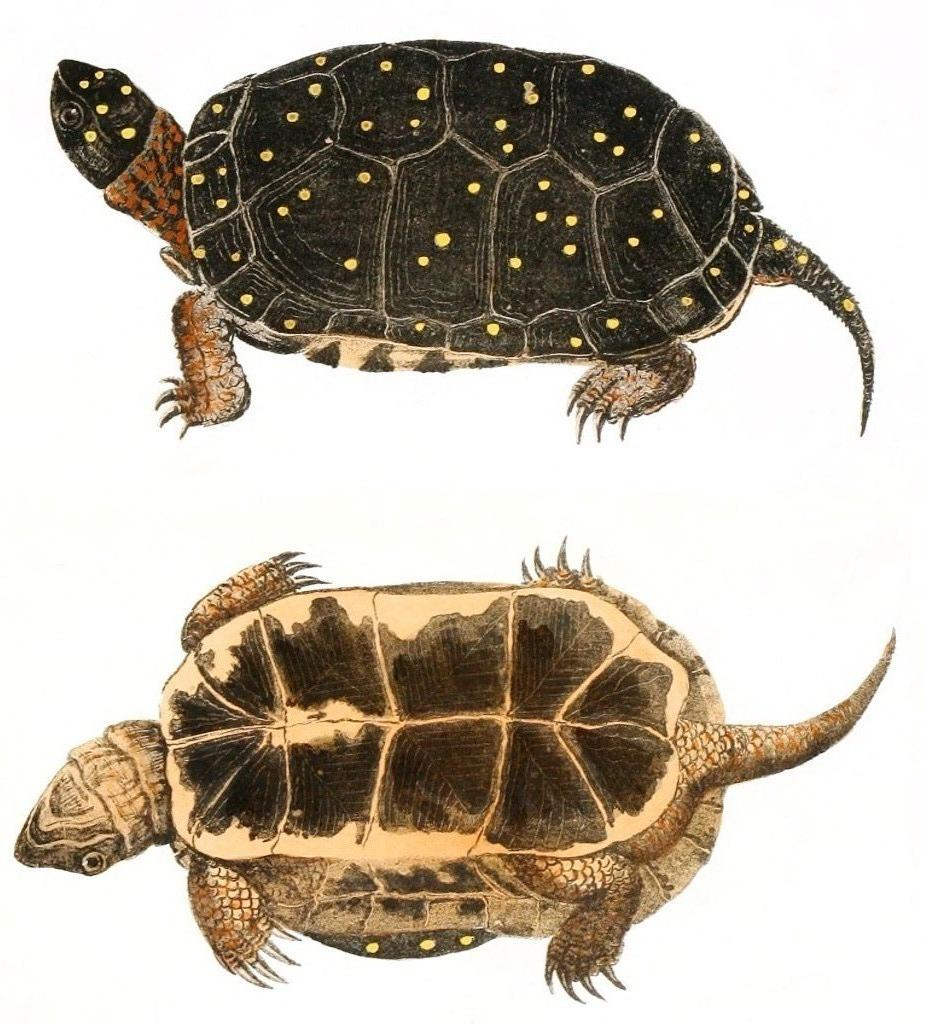
\includegraphics[scale=0.375]{testudines/emydidae/clemmys/1}
\end{center}